%=====================================================================
%  homological_understanding.tex
%  Exactness as a Lens: chain complexes, Mayer-Vietoris, LES on P^1_C.
%  Compile:  latexmk -pdf homological_understanding.tex
%  No shell-escape, no external images, no nonstandard fonts.
%=====================================================================
\documentclass[11pt]{article}

\usepackage[T1]{fontenc}
\usepackage{lmodern}
\usepackage[a4paper,margin=2.2cm]{geometry}
\usepackage{amsmath,amssymb,amsthm,mathtools}
\usepackage{tikz}
\usepackage{tikz-cd}
\usepackage{xcolor}
\usepackage{enumitem}
\usepackage{array}
\usepackage{booktabs}

\usetikzlibrary{arrows.meta,positioning,calc,fit,backgrounds,decorations.markings,decorations.pathmorphing}

%---------------------------------------------------------------------
\definecolor{inkblue}{RGB}{22,32,72}
\definecolor{polered}{RGB}{172,28,40}
\definecolor{zerogreen}{RGB}{18,108,72}
\definecolor{accent}{RGB}{176,104,12}
\definecolor{paper}{RGB}{250,248,240}
\definecolor{faint}{RGB}{120,120,132}

%---------------------------------------------------------------------
\newcommand{\CC}{\mathbb C}
\newcommand{\RR}{\mathbb R}
\newcommand{\ZZ}{\mathbb Z}
\newcommand{\QQ}{\mathbb Q}
\newcommand{\PP}{\mathbb P}
\newcommand{\OO}{\mathcal O}
\newcommand{\FF}{\mathcal F}
\newcommand{\GG}{\mathcal G}
\newcommand{\HH}{\mathcal H}
\newcommand{\CCech}{\check C}
\newcommand{\Hcech}{\check H}
\newcommand{\dR}{\mathrm{dR}}
\newcommand{\im}{\operatorname{im}}
\newcommand{\coker}{\operatorname{coker}}
\newcommand{\kerop}{\operatorname{ker}}
\newcommand{\Hom}{\operatorname{Hom}}
\newcommand{\Ext}{\operatorname{Ext}}
\newcommand{\id}{\operatorname{id}}
\newcommand{\res}{\operatorname{res}}
\newcommand{\Pic}{\operatorname{Pic}}
\newcommand{\Supp}{\operatorname{Supp}}

\newcommand{\slogan}[1]{%
  \begin{center}\setlength{\fboxrule}{0.9pt}%
  \fcolorbox{accent}{paper}{\parbox{0.9\linewidth}{\centering\itshape #1}}%
  \end{center}}
\newcommand{\diagnose}[1]{%
  \par\smallskip\noindent{\color{accent}\textbf{Diagnosis.}}\ \emph{#1}\par\smallskip}

%---------------------------------------------------------------------
%  Geometric-atlas figure styles + numbering
%---------------------------------------------------------------------
\tikzset{
  >=Stealth,
  axisline/.style={inkblue, line width=0.6pt, -{Stealth[length=1.8mm]}},
  loopdir/.style={postaction={decorate},
    decoration={markings, mark=at position 0.62 with {\arrow{Stealth[length=2.2mm]}}}},
  cell/.style={inkblue, font=\small, inner sep=2.5pt, align=center},
}
\newcounter{figcnt}
\newcommand{\figcap}[2]{\refstepcounter{figcnt}\label{#1}\par\smallskip
  {\centering\footnotesize\textbf{Figure~\thefigcnt.}\ \textit{#2}\par}\smallskip}

\theoremstyle{plain}
\newtheorem{proposition}{Proposition}
\newtheorem{lemma}{Lemma}
\theoremstyle{definition}
\newtheorem{remark}{Remark}

\setlist[enumerate]{leftmargin=2.0em, itemsep=2pt, topsep=3pt}
\setlist[itemize]{leftmargin=1.6em, itemsep=2pt, topsep=3pt}

%---------------------------------------------------------------------
\title{\bfseries Exactness as a Lens:\\[2pt]
  Chain Complexes, Mayer--Vietoris, and Long Exact Sequences}
\author{\textsc{A Computation-First Homological Atlas}}
\date{\today}
%---------------------------------------------------------------------

\begin{document}
\maketitle

\begin{center}\itshape\small
A computation-first guide to understanding a mathematical situation by cutting,
comparing, connecting, and gluing.
\end{center}

\medskip
\slogan{A chain complex records what fails to be exact. A short exact sequence
compares three worlds. A long exact sequence is the shadow that comparison casts
on cohomology. Mayer--Vietoris is the art of understanding a global object by
cutting it into local pieces and measuring the obstruction to gluing.}

%=====================================================================
\section{The Situation and the Targets}
%=====================================================================
\noindent\textbf{The situation.} We study
\[
  X=\PP^1_{\CC},
\]
which we read in \emph{two} compatible ways. Topologically $\PP^1_\CC$ is the
real $2$-sphere $S^2$, so it carries de Rham cohomology over $\RR$. Analytically
it is a complex curve carrying the sheaves $\OO$ (holomorphic functions),
$\OO^\times$ (nowhere-zero holomorphic functions), the constant sheaf $\ZZ$, and
the line bundles $\OO(d)$. Both readings use the \emph{same} two-set cover
\[
  U_0=\PP^1\setminus\{\infty\}\cong\CC,\qquad
  U_\infty=\PP^1\setminus\{0\}\cong\CC,\qquad
  U_0\cap U_\infty=\CC^\times\simeq S^1,
\]
with $z$ the coordinate on $U_0$ and $w=1/z$ the coordinate on $U_\infty$. The
pieces $U_0,U_\infty$ are contractible (and Stein); the overlap $\CC^\times$ is
homotopy equivalent to a circle. This single picture --- two disks glued along an
annulus --- is the engine of the whole document. Figure~\ref{fig:cover} shows
this cover both as a sphere and as a Venn diagram.

\begin{center}
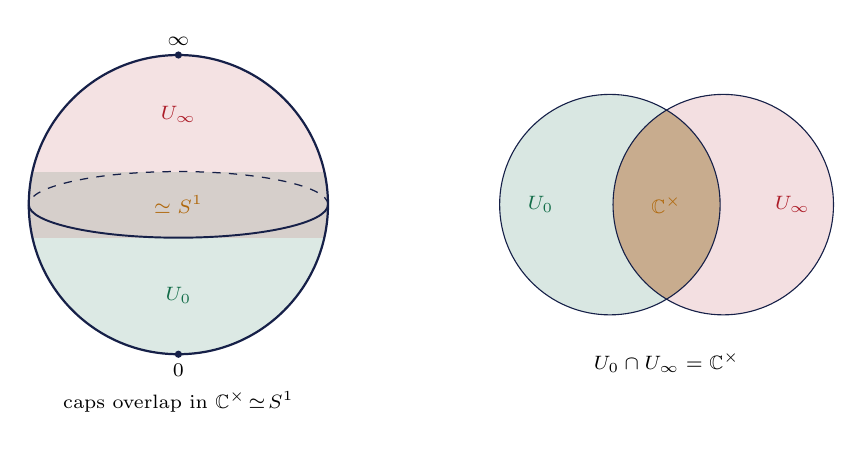
\begin{tikzpicture}
  % ---- left: the sphere S^2 = P^1 as two overlapping caps ----
  \begin{scope}
    \clip (0,0) circle (1.9);
    \fill[zerogreen, fill opacity=0.15] (-1.9,-1.9) rectangle (1.9,0.42);
    \fill[polered,  fill opacity=0.13] (-1.9,-0.42) rectangle (1.9,1.9);
  \end{scope}
  \draw[inkblue, line width=0.8pt] (0,0) circle (1.9);
  \draw[inkblue, dashed, line width=0.45pt] (1.9,0) arc[start angle=0, end angle=180, x radius=1.9, y radius=0.42];
  \draw[inkblue, line width=0.7pt] (1.9,0) arc[start angle=0, end angle=-180, x radius=1.9, y radius=0.42];
  \fill[inkblue] (0,-1.9) circle (1.3pt); \node[below=0pt, font=\scriptsize] at (0,-1.9) {$0$};
  \fill[inkblue] (0, 1.9) circle (1.3pt); \node[above=0pt, font=\scriptsize] at (0, 1.9) {$\infty$};
  \node[zerogreen, font=\scriptsize] at (0,-1.15) {$U_0$};
  \node[polered,  font=\scriptsize] at (0, 1.15) {$U_\infty$};
  \node[accent,   font=\scriptsize] at (0, 0) {$\simeq S^1$};
  \node[font=\scriptsize] at (0,-2.5) {caps overlap in $\CC^\times\!\simeq\! S^1$};
  % ---- right: the Venn companion ----
  \begin{scope}[shift={(6.2,0)}]
    \fill[zerogreen, fill opacity=0.16] (-0.72,0) circle (1.4);
    \fill[polered,  fill opacity=0.14] ( 0.72,0) circle (1.4);
    \begin{scope}\clip (-0.72,0) circle (1.4);
      \fill[accent, fill opacity=0.30] (0.72,0) circle (1.4);\end{scope}
    \draw[inkblue] (-0.72,0) circle (1.4);
    \draw[inkblue] ( 0.72,0) circle (1.4);
    \node[zerogreen, font=\scriptsize] at (-1.6,0) {$U_0$};
    \node[polered,  font=\scriptsize] at ( 1.6,0) {$U_\infty$};
    \node[accent, font=\scriptsize] at (0,0) {$\CC^\times$};
    \node[font=\scriptsize] at (0,-2.0) {$U_0\cap U_\infty=\CC^\times$};
  \end{scope}
\end{tikzpicture}
\figcap{fig:cover}{The cover of $\PP^1=S^2$: two contractible caps $U_0$ (around
$0$) and $U_\infty$ (around $\infty$) overlapping in the equatorial annulus
$\CC^\times\simeq S^1$ --- the homotopy model that drives every computation
below. \emph{Left}: as a sphere; \emph{right}: as a Venn diagram. (Supports
\S1, \S7, \S8.)}
\end{center}

\begin{remark}[Stated assumptions]\label{rmk:assume}
The situation slot was delivered empty. We fix $X=\PP^1_\CC$ because it lets
\emph{every} homological tool below be computed in closed form and unifies all
four requested micro-examples ($S^1$, $S^2$, $\PP^1$, line bundles) in one
space. De Rham statements use $\RR$ coefficients; \v Cech/sheaf statements use
the indicated sheaf. We use the cover $\{U_0,U_\infty\}$ throughout; it is a
\emph{Leray} (acyclic) cover for the coherent sheaves below, so \v Cech
cohomology equals sheaf cohomology. Where a surjectivity uses a smooth partition
of unity we say so explicitly, and we flag where the holomorphic world has none.
\end{remark}

\medskip\noindent\textbf{The targets of understanding.}
\begin{enumerate}
  \item the relevant chain/cochain complexes (de Rham on $X$; \v Cech on
        $\{U_0,U_\infty\}$);
  \item the local pieces $U_0$, $U_\infty$, and the overlap $U_0\cap U_\infty=\CC^\times$;
  \item the short exact sequence comparing global data with local data;
  \item the Mayer--Vietoris sequence;
  \item the connecting homomorphism $\delta$;
  \item the resulting long exact sequence;
  \item the concrete groups $H^\bullet_\dR(\PP^1)$, $H^\bullet(\PP^1,\OO)$,
        $\Pic(\PP^1)$;
  \item the geometric meaning of every kernel, image, cokernel, and obstruction.
\end{enumerate}
We do not treat homological algebra as formal decoration. We use it as a
microscope: each exact sequence is pointed at a specific target and made to
reveal it.

%=====================================================================
\section{Chain Complexes: The Basic Machine}
%=====================================================================
\noindent\textbf{The de Rham cochain complex.} On the smooth $2$-manifold
$X=\PP^1\cong S^2$,
\[
  0\longrightarrow \Omega^0(X)\xrightarrow{\,d\,}\Omega^1(X)
  \xrightarrow{\,d\,}\Omega^2(X)\longrightarrow 0,
\]
where $\Omega^k(X)$ is the $\RR$-vector space of smooth $k$-forms and $d$ is the
exterior derivative. In a local coordinate, $\Omega^0$ is functions $f$,
$\Omega^1$ is $a\,dx+b\,dy$, $\Omega^2$ is $h\,dx\wedge dy$, and
\[
  d^2=0
  \qquad\bigl(\text{e.g. } d(df)=\partial_{xy}f\,dx\wedge dy-\partial_{yx}f\,dy\wedge dx=0\bigr).
\]
A form $\omega$ is a \emph{cocycle} (closed) if $d\omega=0$, a \emph{coboundary}
(exact) if $\omega=d\eta$. The cohomology is
\[
  H^n_\dR(X)=\frac{\kerop(d:\Omega^n\to\Omega^{n+1})}
                  {\im(d:\Omega^{n-1}\to\Omega^{n})}
  =\frac{\text{closed }n\text{-forms}}{\text{exact }n\text{-forms}} .
\]

\medskip\noindent\textbf{The \v Cech cochain complex.} For the two-set cover
$\mathfrak U=\{U_0,U_\infty\}$ and a sheaf $\FF$,
\[
  0\longrightarrow \CCech^0(\mathfrak U,\FF)\xrightarrow{\,\delta\,}
  \CCech^1(\mathfrak U,\FF)\longrightarrow 0,\qquad
  \CCech^0=\FF(U_0)\oplus\FF(U_\infty),\quad
  \CCech^1=\FF(U_0\cap U_\infty),
\]
with
\[
  \delta(f_0,f_\infty)=\bigl(f_\infty-f_0\bigr)\big|_{U_0\cap U_\infty}.
\]
Because the cover has only two sets there are no triple overlaps, so
$\CCech^{\ge2}=0$ and $\delta^2=0$ \emph{trivially}; the cocycle condition in
degree $\ge2$ is vacuous. Then
\[
  \Hcech^0(\mathfrak U,\FF)=\kerop\delta=\{(f_0,f_\infty):f_0=f_\infty\text{ on }U_0\cap U_\infty\}=\FF(X),
  \qquad
  \Hcech^1(\mathfrak U,\FF)=\coker\delta .
\]

\slogan{Cohomology measures closed objects modulo exact objects.}

\noindent Concretely on $\CC^\times$: $d\theta$ is closed but not exact ($\theta$
is not a global function), so $[d\theta]\neq0$ in $H^1_\dR(\CC^\times)$. That one
nonzero class is the seed from which the $H^2$ of $\PP^1$ will grow. The overlap
and its winding class are drawn in Figure~\ref{fig:annulus}.

\begin{center}
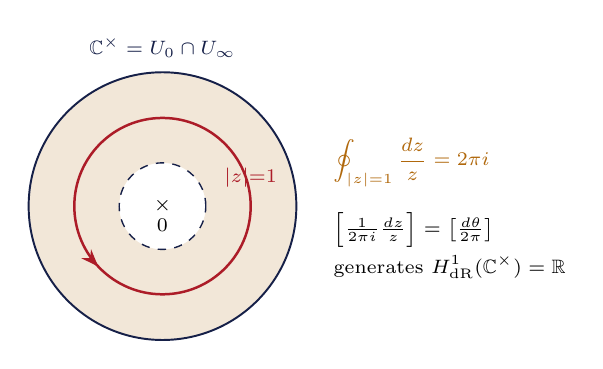
\begin{tikzpicture}
  \fill[accent!16, even odd rule] (0,0) circle (1.7) (0,0) circle (0.55);
  \draw[inkblue, line width=0.7pt] (0,0) circle (1.7);
  \draw[inkblue, dashed, line width=0.5pt] (0,0) circle (0.55);
  \node[font=\scriptsize] at (0,0) {$\times$};
  \node[font=\scriptsize, below=1pt] at (0,0) {$0$};
  \draw[polered, line width=0.9pt, loopdir] (0,0) circle (1.12);
  \node[polered, font=\scriptsize] at (1.12,0.36) {$|z|{=}1$};
  \node[inkblue, font=\scriptsize] at (0,2.02) {$\CC^\times=U_0\cap U_\infty$};
  \node[accent, font=\scriptsize, right] at (2.05,0.55) {$\displaystyle\oint_{|z|=1}\frac{dz}{z}=2\pi i$};
  \node[font=\scriptsize, right, align=left] at (2.05,-0.5)
    {$\Bigl[\tfrac{1}{2\pi i}\tfrac{dz}{z}\Bigr]=\bigl[\tfrac{d\theta}{2\pi}\bigr]$\\[2pt]
     generates $H^1_\dR(\CC^\times)=\RR$};
\end{tikzpicture}
\figcap{fig:annulus}{The overlap $\CC^\times\simeq S^1$ as a punctured disk. The
oriented loop $|z|=1$ carries the winding class $[\tfrac{1}{2\pi i}\tfrac{dz}{z}]
=[\tfrac{d\theta}{2\pi}]$, the single generator of $H^1_\dR(\CC^\times)=\RR$ that
the connecting map will promote to the area class of $\PP^1$. (Supports \S2,
Example~C.)}
\end{center}

%=====================================================================
\section{Exactness as a Diagnostic}
%=====================================================================
A pair of maps is \emph{exact} at the middle term when image equals kernel:
\[
  A\xrightarrow{f}B\xrightarrow{g}C \ \text{ is exact at }B
  \quad\Longleftrightarrow\quad \im f=\kerop g .
\]
We read each exact sequence as a measurement:
\begin{itemize}
  \item $\kerop g$ collects the elements of $B$ that satisfy the
        \emph{compatibility constraint} imposed by $g$;
  \item $\im f$ collects the elements of $B$ that are \emph{already produced} by
        $A$ (``already glued'');
  \item exactness says: \emph{every} constrained element is produced --- no more,
        no less;
  \item failure of exactness, measured by $\kerop g/\im f$, is an
        \emph{obstruction}: a constrained element that is \emph{not} produced.
\end{itemize}
Every exact sequence in this document is accompanied by its maps, its kernel, its
image, its connecting map (when present), and a one-line diagnosis of what the
obstruction means.

%=====================================================================
\section{Short Exact Sequences of Complexes}
%=====================================================================
A \emph{short exact sequence of cochain complexes} is a triple of complexes with
degreewise maps
\[
  0\longrightarrow A^\bullet\xrightarrow{\,i\,}B^\bullet\xrightarrow{\,p\,}C^\bullet\longrightarrow 0
\]
such that in every degree the row is exact and the maps commute with the
differentials:
\[
\begin{tikzcd}[row sep=2.2em, column sep=2.2em]
0 \arrow[r] & A^n \arrow[r,"i^n"] \arrow[d,"d_A"]
& B^n \arrow[r,"p^n"] \arrow[d,"d_B"]
& C^n \arrow[r] \arrow[d,"d_C"]
& 0 \\
0 \arrow[r] & A^{n+1} \arrow[r,"i^{n+1}"]
& B^{n+1} \arrow[r,"p^{n+1}"]
& C^{n+1} \arrow[r]
& 0
\end{tikzcd}
\]
Exactness of each row says: $i^n$ is injective, $\im i^n=\kerop p^n$, and $p^n$
is surjective. Commutativity $d_B i=i\,d_A$ and $p\,d_B=d_C\,p$ says the three
differentials are \emph{one differential seen in three worlds}. This is exactly
what lets the cohomologies communicate.

\diagnose{$A^\bullet$ is the sub-world sitting inside $B^\bullet$; $C^\bullet$ is
the quotient world $B^\bullet/A^\bullet$. The sequence compares ``global'' and
``local'' data in our case: $A^\bullet=\Omega^\bullet(X)$, $B^\bullet=
\Omega^\bullet(U_0)\oplus\Omega^\bullet(U_\infty)$, $C^\bullet=\Omega^\bullet(\CC^\times)$
(Section~7).}

\begin{proposition}[Zig-zag]\label{prop:zigzag}
A short exact sequence of complexes induces a long exact sequence in cohomology,
\[
  \cdots\to H^n(A^\bullet)\xrightarrow{i_*}H^n(B^\bullet)\xrightarrow{p_*}
  H^n(C^\bullet)\xrightarrow{\ \delta\ }H^{n+1}(A^\bullet)\to\cdots,
\]
where $\delta$ is the connecting homomorphism constructed in Section~5.
\end{proposition}

%=====================================================================
\section{The Connecting Homomorphism}
%=====================================================================
We \emph{construct} $\delta\colon H^n(C^\bullet)\to H^{n+1}(A^\bullet)$; we do not
merely name it. The construction is a chase through the diagram
\[
\begin{tikzcd}[row sep=2.4em, column sep=2.6em]
& B^n \arrow[r,"p^n", two heads] \arrow[d,"d_B"] & C^n \arrow[d,"d_C"] \\
A^{n+1} \arrow[r,"i^{n+1}"', hook] & B^{n+1} \arrow[r,"p^{n+1}"] & C^{n+1}.
\end{tikzcd}
\]
\begin{enumerate}
  \item Start with a class $[c]\in H^n(C^\bullet)$, represented by a cocycle
        $c\in C^n$ with $d_Cc=0$.
  \item Since $p^n$ is surjective, choose a lift $b\in B^n$ with $p^n(b)=c$.
  \item Push down: $d_Bb\in B^{n+1}$.
  \item Compute its image: $p^{n+1}(d_Bb)=d_C\,p^n(b)=d_Cc=0$, using commutativity
        and step~1.
  \item Hence $d_Bb\in\kerop p^{n+1}=\im i^{n+1}$ by exactness.
  \item Since $i^{n+1}$ is injective, there is a \emph{unique} $a\in A^{n+1}$ with
        $i^{n+1}(a)=d_Bb$.
  \item Define $\delta([c])=[a]\in H^{n+1}(A^\bullet)$.
\end{enumerate}

\noindent\textbf{$a$ is a cocycle.} Apply $i^{n+2}$ to $d_Aa$: by commutativity
$i^{n+2}(d_Aa)=d_B\,i^{n+1}(a)=d_B(d_Bb)=0$. As $i^{n+2}$ is injective, $d_Aa=0$.

\noindent\textbf{Independence of the lift $b$.} Another lift is $b'=b+i(a')$ for
some $a'\in A^n$ (since $p(b'-b)=0$). Then $d_Bb'=d_Bb+i(d_Aa')$, so the new
$a$ is $a+d_Aa'$, and $[a+d_Aa']=[a]$.

\noindent\textbf{Independence of the representative $c$.} Replacing $c$ by
$c+d_C\gamma$ ($\gamma\in C^{n-1}$): lift $\gamma$ to $\beta\in B^{n-1}$, then
$b+d_B\beta$ lifts $c+d_C\gamma$ and $d_B(b+d_B\beta)=d_Bb$, so $a$ is unchanged.
Thus $\delta$ is a well-defined homomorphism.

\slogan{The connecting homomorphism measures the obstruction to lifting a closed
object in $C^\bullet$ to a closed object in $B^\bullet$.}

\diagnose{In our Mayer--Vietoris setting, $C^\bullet=\Omega^\bullet(\CC^\times)$:
$\delta$ takes a closed form on the overlap $\CC^\times$ and returns the global
class on $\PP^1$ obstructing the splitting of that overlap form into a
\emph{difference of} forms living on $U_0$ and $U_\infty$. A nonzero $\delta$
means the overlap form cannot be untwisted into local pieces.}

%=====================================================================
\section{The Long Exact Sequence}
%=====================================================================
Proposition~\ref{prop:zigzag} gives, for any short exact sequence of complexes,
\[
  \cdots\to H^n(A^\bullet)\xrightarrow{i_*}H^n(B^\bullet)\xrightarrow{p_*}
  H^n(C^\bullet)\xrightarrow{\delta}H^{n+1}(A^\bullet)\xrightarrow{i_*}
  H^{n+1}(B^\bullet)\to\cdots
\]
Read segment by segment:
\begin{itemize}
  \item \emph{Exact at $H^n(B)$:} $\im i_*=\kerop p_*$. A class on $B$ dies in $C$
        iff it comes from $A$.
  \item \emph{Exact at $H^n(C)$:} $\im p_*=\kerop\delta$. A class on $C$ lifts to
        $B$ iff its obstruction $\delta$ vanishes.
  \item \emph{Exact at $H^{n+1}(A)$:} $\im\delta=\kerop i_*$. A class on $A$ is a
        genuine obstruction (in the image of $\delta$) iff it becomes trivial in
        $B$.
\end{itemize}
We now specialize the abstract $A,B,C$ to the geometric pieces of $\PP^1$.

%=====================================================================
\section{Mayer--Vietoris from a Short Exact Sequence}
%=====================================================================
Let $X=U\cup V$; here $U=U_0$, $V=U_\infty$, $U\cap V=\CC^\times$. The
\emph{Mayer--Vietoris short exact sequence of de Rham complexes} is
\[
  0\longrightarrow \Omega^\bullet(X)\xrightarrow{\,r\,}
  \Omega^\bullet(U)\oplus\Omega^\bullet(V)\xrightarrow{\,s\,}
  \Omega^\bullet(U\cap V)\longrightarrow 0,
\]
\[
  r(\omega)=(\omega|_U,\ \omega|_V),
  \qquad
  s(\alpha,\beta)=\alpha|_{U\cap V}-\beta|_{U\cap V}.
\]
\textbf{Exactness, checked term by term.}
\begin{itemize}
  \item \emph{$r$ injective.} If $\omega|_U=0$ and $\omega|_V=0$ then $\omega=0$,
        since $\{U,V\}$ covers $X$ and a form is determined by its restrictions.
        ($\kerop r=0$: \emph{compatibility forces nothing extra}.)
  \item \emph{$s\circ r=0$.} $s(r\omega)=\omega|_{U\cap V}-\omega|_{U\cap V}=0$:
        the two restrictions of a global form agree on the overlap.
  \item \emph{$\kerop s=\im r$.} If $s(\alpha,\beta)=0$ then $\alpha=\beta$ on
        $U\cap V$, so $\alpha,\beta$ \emph{glue} to a global form $\omega$ with
        $r\omega=(\alpha,\beta)$. (This is the gluing axiom in algebraic dress.)
  \item \emph{$s$ surjective.} Given $\gamma\in\Omega^k(U\cap V)$, pick a smooth
        partition of unity $\{\rho_U,\rho_V\}$ subordinate to $\{U,V\}$
        ($\rho_U+\rho_V=1$, $\Supp\rho_U\subset U$, $\Supp\rho_V\subset V$). Set
        \[
          \alpha=\rho_V\,\gamma\ \text{(extended by $0$ to }U),\qquad
          \beta=-\rho_U\,\gamma\ \text{(extended by $0$ to }V).
        \]
        These are smooth because $\rho_V$ vanishes near $U\setminus V$ and
        $\rho_U$ vanishes near $V\setminus U$. On the overlap
        $\alpha-\beta=(\rho_U+\rho_V)\gamma=\gamma$, so $s(\alpha,\beta)=\gamma$.
\end{itemize}
\begin{remark}[Where the partition of unity is essential]
Surjectivity of $s$ is the \emph{only} step needing a partition of unity, and it
is genuinely smooth: there is \textbf{no holomorphic partition of unity}. For
holomorphic data one must instead control surjectivity by hand or pass to the
\v Cech complex, where $\delta$ onto $\CCech^1$ is automatic because $\CCech^1$ is
the top term (Section~2). This is the precise point where the smooth and
holomorphic stories diverge.
\end{remark}

\noindent Feeding this short exact sequence into Proposition~\ref{prop:zigzag}
gives the \textbf{Mayer--Vietoris long exact sequence}
\[
  \cdots\to H^k_\dR(X)\xrightarrow{r_*}H^k_\dR(U)\oplus H^k_\dR(V)
  \xrightarrow{s_*}H^k_\dR(U\cap V)\xrightarrow{\ \delta\ }H^{k+1}_\dR(X)\to\cdots
\]
For sheaf cohomology the analogous sequence (no partition of unity) is the
\v Cech--Mayer--Vietoris sequence
\[
  0\to \FF(X)\to \FF(U)\oplus \FF(V)\to \FF(U\cap V)\to
  H^1(X,\FF)\to H^1(U,\FF)\oplus H^1(V,\FF)\to\cdots
\]
whose maps are $f\mapsto(f|_U,f|_V)$ and $(f,g)\mapsto f|_{U\cap V}-g|_{U\cap V}$.

%=====================================================================
\section{Explicit Mayer--Vietoris Computation for $\PP^1$}
%=====================================================================
\textbf{Cohomology of the pieces.} $U_0\cong\CC$ and $U_\infty\cong\CC$ are
contractible, so
\[
  H^0_\dR(U_0)=H^0_\dR(U_\infty)=\RR,\qquad H^{\ge1}_\dR(U_0)=H^{\ge1}_\dR(U_\infty)=0 .
\]
The overlap $U_0\cap U_\infty=\CC^\times\simeq S^1$ has
\[
  H^0_\dR(\CC^\times)=\RR,\qquad H^1_\dR(\CC^\times)=\RR\cdot[d\theta],\qquad H^{\ge2}=0 .
\]
\textbf{The sequence with numbers.} Writing $\delta^k$ for the connecting maps,
\[
\begin{tikzcd}[column sep=1.45em, row sep=0.3em]
0 \arrow[r] & H^0(\PP^1) \arrow[r,"r_*"] & \RR^2 \arrow[r,"s^0"] & \RR
   \arrow[r,"\delta^0"] & H^1(\PP^1) \arrow[r] & 0
   \arrow[r] & \RR \arrow[r,"\delta^1"] & H^2(\PP^1) \arrow[r] & 0 .
\end{tikzcd}
\]
\emph{Degree $0$.} $s^0(a,b)=a-b$ (constants differ on the connected overlap).
Then $\kerop s^0=\{a=b\}\cong\RR$, so $H^0(\PP^1)=\im r_*=\kerop s^0=\RR$: the
sphere is connected. And $s^0$ is \emph{surjective}, so $\im s^0=\RR=\kerop\delta^0$,
forcing $\delta^0=0$.

\emph{Degree $1$.} Exactness at $H^1(\PP^1)$ reads $\im\delta^0=\kerop r_*$. Since
$\delta^0=0$ and $r_*\colon H^1(\PP^1)\to H^1(U_0)\oplus H^1(U_\infty)=0$, we get
\[
  H^1(\PP^1)=\im\delta^0=0 .
\]
\emph{Degree $2$.} The tail is $0\xrightarrow{s^1}\RR\xrightarrow{\delta^1}H^2(\PP^1)\to0$.
The incoming $s^1$ has source $H^1(U_0)\oplus H^1(U_\infty)=0$, so $\kerop\delta^1
=\im s^1=0$ ($\delta^1$ injective); the outgoing map lands in
$H^2(U_0)\oplus H^2(U_\infty)=0$, so $\im\delta^1=H^2(\PP^1)$ ($\delta^1$
surjective). Therefore
\[
  \boxed{\ \delta^1\colon H^1_\dR(\CC^\times)\xrightarrow{\ \cong\ }H^2_\dR(\PP^1)\ },
  \qquad H^2_\dR(\PP^1)=\RR .
\]
\diagnose{The entire second cohomology of $\PP^1=S^2$ is \emph{created by the
connecting map} out of the single winding class $[d\theta]$ on the overlap
circle. The fundamental class of the sphere is the obstruction to splitting
$d\theta$ across the two disks. We make this completely explicit next.}

We have recovered $H^\bullet_\dR(\PP^1)=(\RR,0,\RR)$, with Euler characteristic
$1-0+1=2=\chi(S^2)$, consistent with $\chi(U_0)+\chi(U_\infty)-\chi(\CC^\times)=1+1-0$. The whole
computation reads off the staircase in Figure~\ref{fig:staircase}.

\begin{center}
\resizebox{0.96\textwidth}{!}{%
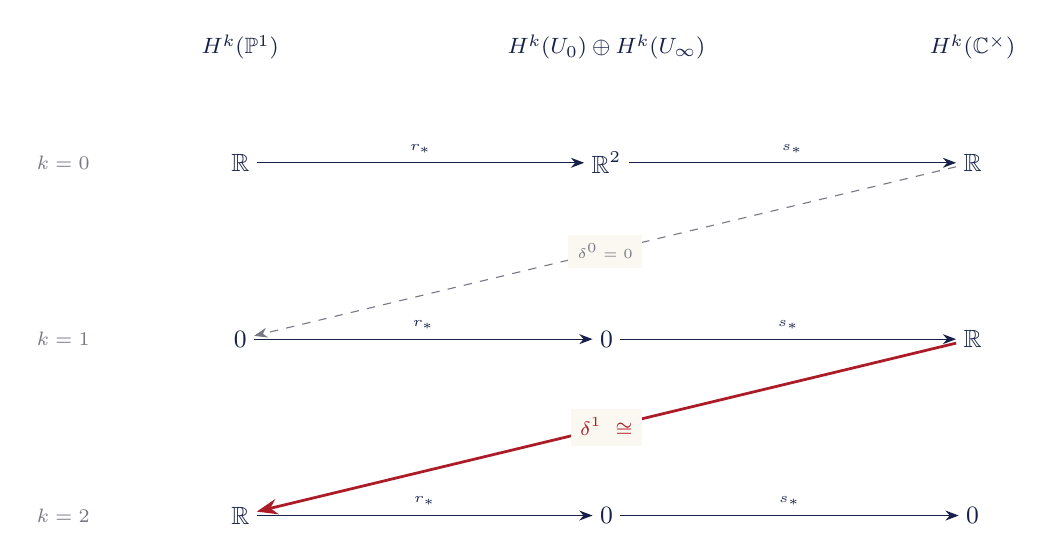
\begin{tikzpicture}[x=1.55cm, y=1.4cm]
  \node[cell, font=\footnotesize] at (0, 1.05) {$H^k(\PP^1)$};
  \node[cell, font=\footnotesize] at (3, 1.05) {$H^k(U_0)\oplus H^k(U_\infty)$};
  \node[cell, font=\footnotesize] at (6, 1.05) {$H^k(\CC^\times)$};
  \node[faint, font=\scriptsize] at (-1.45, 0)   {$k=0$};
  \node[faint, font=\scriptsize] at (-1.45,-1.6) {$k=1$};
  \node[faint, font=\scriptsize] at (-1.45,-3.2) {$k=2$};
  \node[cell] (X0) at (0,0) {$\RR$};    \node[cell] (M0) at (3,0) {$\RR^2$}; \node[cell] (V0) at (6,0) {$\RR$};
  \node[cell] (X1) at (0,-1.6) {$0$};   \node[cell] (M1) at (3,-1.6) {$0$};  \node[cell] (V1) at (6,-1.6) {$\RR$};
  \node[cell] (X2) at (0,-3.2) {$\RR$}; \node[cell] (M2) at (3,-3.2) {$0$};  \node[cell] (V2) at (6,-3.2) {$0$};
  \foreach \a/\b/\c in {X0/M0/V0, X1/M1/V1, X2/M2/V2}{
    \draw[->, inkblue] (\a)--(\b) node[midway, above, font=\tiny]{$r_*$};
    \draw[->, inkblue] (\b)--(\c) node[midway, above, font=\tiny]{$s_*$};
  }
  \draw[->, faint, dashed] (V0)--(X1) node[midway, fill=paper, font=\tiny]{$\delta^0=0$};
  \draw[->, polered, line width=1pt] (V1)--(X2)
        node[midway, fill=paper, font=\scriptsize, text=polered]{$\delta^1\ \cong$};
\end{tikzpicture}}
\figcap{fig:staircase}{The Mayer--Vietoris long exact sequence as a staircase for
$\PP^1$. Horizontal maps are restriction $r_*$ and difference $s_*$; the
\textcolor{polered}{red} diagonal $\delta^1$ is the connecting isomorphism
$H^1(\CC^\times)=\RR\xrightarrow{\cong}H^2(\PP^1)=\RR$ that \emph{manufactures}
the top cohomology of the sphere out of the overlap circle, while $\delta^0=0$.
(Supports \S6, \S8.)}
\end{center}

%=====================================================================
\section{A Diagram Chase: Where the Obstruction Lives}
%=====================================================================
We chase $\delta^1$ on the generator $\gamma=\tfrac{1}{2\pi}\,d\theta\in
\Omega^1(\CC^\times)$ (equivalently the class of $\tfrac{1}{2\pi i}\tfrac{dz}{z}$,
since $\tfrac{dz}{z}=\tfrac{dr}{r}+i\,d\theta$ and $\tfrac{dr}{r}=d(\log r)$ is
exact). Fix a radial partition of unity $\rho_0+\rho_\infty=1$ with $\rho_\infty=0$
near $z=0$ and $\rho_\infty=1$ near $z=\infty$. The chase
\[
  \gamma\in C^1
  \ \leadsto\ b=(\rho_\infty\gamma,\,-\rho_0\gamma)\in B^1
  \ \leadsto\ d_Bb\in B^2
  \ \leadsto\ a\in A^2=\Omega^2(\PP^1)
  \ \leadsto\ [a]\in H^2(\PP^1)
\]
runs as follows.
\begin{itemize}
  \item \emph{$\gamma\leadsto b$:} $s(b)=\rho_\infty\gamma-(-\rho_0\gamma)
        =(\rho_0+\rho_\infty)\gamma=\gamma$, so $b$ is a lift of $\gamma$ (step~2 of
        Section~5).
  \item \emph{$b\leadsto d_Bb$:} $d_Bb=\bigl(d(\rho_\infty\gamma),\,-d(\rho_0\gamma)\bigr)$.
        On the overlap, $d(\rho_\infty\gamma)-(-d(\rho_0\gamma))=d\gamma=0$, so both
        components agree there: $d_Bb\in\kerop s=\im r$.
  \item \emph{$d_Bb\leadsto a$:} the unique global form with $r(a)=d_Bb$ is
        \[
          a=d(\rho_\infty\gamma)=d\rho_\infty\wedge\gamma
          \quad(\text{since } \rho_\infty d\gamma=0),
        \]
        extended by $0$ outside the overlap (it is supported where $d\rho_\infty\neq0$,
        an annulus inside $\CC^\times$).
  \item \emph{$a\leadsto[a]$:} $a$ is closed ($da=d(d(\rho_\infty\gamma))=0$), hence
        defines $\delta^1[\gamma]=[a]\in H^2(\PP^1)$.
\end{itemize}
\textbf{It is the generator.} In polar coordinates $\gamma=\tfrac{1}{2\pi}d\theta$
and $\rho_\infty=\rho_\infty(r)$, so
\[
  \int_{\PP^1}a=\int_{\PP^1}d\rho_\infty\wedge\tfrac{1}{2\pi}d\theta
  =\int_0^\infty\!\!\int_0^{2\pi}\rho_\infty'(r)\,\tfrac{1}{2\pi}\,d\theta\,dr
  =\int_0^\infty\rho_\infty'(r)\,dr=\rho_\infty(\infty)-\rho_\infty(0)=1 .
\]
Thus $\delta^1[\gamma]$ is the positively oriented generator of $H^2_\dR(\PP^1)$.
Figure~\ref{fig:partition} shows this construction geometrically.

\begin{center}
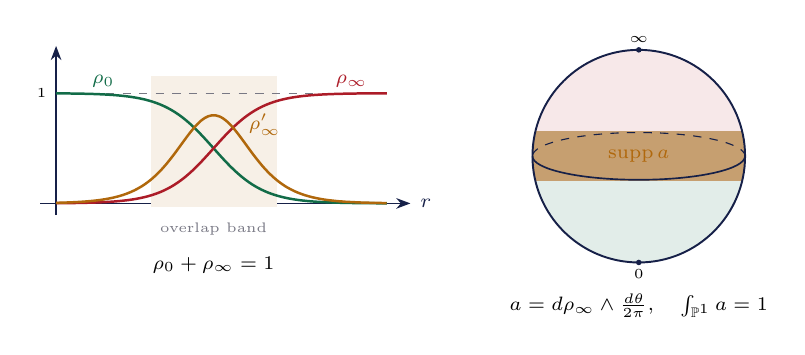
\begin{tikzpicture}
  % (a) partition of unity + derivative bump, as functions of r
  \draw[axisline] (-0.2,0) -- (4.5,0) node[right, font=\scriptsize]{$r$};
  \draw[axisline] (0,-0.15) -- (0,2.0);
  \fill[accent!10] (1.2,-0.05) rectangle (2.8,1.62);
  \draw[faint, dashed] (0,1.4) -- (4.2,1.4); \node[left, font=\tiny] at (0,1.4) {$1$};
  \draw[zerogreen, line width=0.9pt, smooth, samples=80, domain=0:4.2]
        plot (\x, {1.4-1.4/(1+exp(-3.2*(\x-2)))});
  \draw[polered, line width=0.9pt, smooth, samples=80, domain=0:4.2]
        plot (\x, {1.4/(1+exp(-3.2*(\x-2)))});
  \draw[accent, line width=0.9pt, smooth, samples=90, domain=0:4.2]
        plot (\x, {1.4*3.2*(1/(1+exp(-3.2*(\x-2))))*(1-1/(1+exp(-3.2*(\x-2))))});
  \node[zerogreen, font=\scriptsize] at (0.6,1.55) {$\rho_0$};
  \node[polered,  font=\scriptsize] at (3.75,1.55) {$\rho_\infty$};
  \node[accent,   font=\scriptsize] at (2.65,1.0) {$\rho_\infty'$};
  \node[font=\tiny, faint] at (2.0,-0.32) {overlap band};
  \node[font=\scriptsize] at (2.0,-0.78) {$\rho_0+\rho_\infty=1$};
  % (b) the supported 2-form on the sphere
  \begin{scope}[shift={(7.4,0.6)}]
    \begin{scope}\clip (0,0) circle (1.35);
      \fill[zerogreen, fill opacity=0.12] (-1.35,-1.35) rectangle (1.35,0.32);
      \fill[polered,  fill opacity=0.10] (-1.35,-0.32) rectangle (1.35,1.35);
      \fill[accent,   fill opacity=0.5 ] (-1.35,-0.32) rectangle (1.35,0.32);
    \end{scope}
    \draw[inkblue, line width=0.7pt] (0,0) circle (1.35);
    \draw[inkblue, dashed, line width=0.4pt] (1.35,0) arc[start angle=0,end angle=180,x radius=1.35,y radius=0.3];
    \draw[inkblue, line width=0.6pt] (1.35,0) arc[start angle=0,end angle=-180,x radius=1.35,y radius=0.3];
    \fill[inkblue] (0,-1.35) circle (1pt); \node[font=\tiny, below=-1pt] at (0,-1.35){$0$};
    \fill[inkblue] (0, 1.35) circle (1pt); \node[font=\tiny, above=-1pt] at (0, 1.35){$\infty$};
    \node[accent, font=\scriptsize] at (0,0) {$\operatorname{supp}a$};
    \node[font=\scriptsize] at (0,-1.9) {$a=d\rho_\infty\wedge\tfrac{d\theta}{2\pi},\quad \int_{\PP^1}a=1$};
  \end{scope}
\end{tikzpicture}
\figcap{fig:partition}{The geometry of the connecting map. \emph{Left}: a radial
partition of unity $\rho_0+\rho_\infty=1$; the derivative $\rho_\infty'$ is a bump
supported in the overlap band. \emph{Right}: the resulting obstruction $2$-form
$a=d\rho_\infty\wedge\tfrac{d\theta}{2\pi}$ lives \emph{only} in the equatorial
band and integrates to $1$, generating $H^2_\dR(\PP^1)$. (Supports \S9.)}
\end{center}

\slogan{A class on the overlap $U\cap V$ may fail to come from compatible classes
on $U$ and $V$. The connecting map records that failure as a global cohomology
class on $X$.}

%=====================================================================
\section{Relation to Gluing}
%=====================================================================
\slogan{Exactness is the algebra of gluing.}
\noindent The dictionary:
\begin{itemize}
  \item \textbf{kernel} $=$ \emph{compatibility} (data that agree where they
        overlap);
  \item \textbf{image} $=$ \emph{already glued} (data that genuinely come from a
        global object);
  \item \textbf{cokernel} $=$ \emph{obstruction} (compatible-looking data with no
        global origin);
  \item \textbf{connecting map} $=$ the \emph{boundary of a failed gluing attempt}
        (Section~9: $\delta[\gamma]=[d(\rho_\infty\gamma)]$ is literally the
        derivative of a partial, non-global, gluing).
\end{itemize}

\noindent\textbf{Line bundles as a degree-$1$ \v Cech class.} A holomorphic line
bundle is glued from trivial bundles $U_\alpha\times\CC$ by transition functions
$g_{\alpha\beta}\in\OO^\times(U_\alpha\cap U_\beta)$ satisfying the cocycle
condition on triple overlaps,
\[
  g_{\alpha\beta}\,g_{\beta\gamma}\,g_{\gamma\alpha}=1 ,
\]
which is precisely the degree-$1$ \v Cech cocycle equation
$\delta\bigl((g_{\alpha\beta})\bigr)=1$ for the multiplicative sheaf $\OO^\times$.
Changing trivializations $g_{\alpha\beta}\mapsto g_{\alpha\beta}\cdot
(h_\beta/h_\alpha)$ with $h_\alpha\in\OO^\times(U_\alpha)$ alters the cocycle by a
\emph{coboundary}. Hence isomorphism classes of line bundles form
\[
  \boxed{\ \Pic(X)=\Hcech^1(X,\OO^\times)\ }.
\]

\noindent\textbf{Computing $\Pic(\PP^1)$ by a long exact sequence.} The
exponential sheaf sequence on the complex manifold $\PP^1$,
\[
\begin{tikzcd}[column sep=2.2em]
0 \arrow[r] & \ZZ \arrow[r,"2\pi i"] & \OO \arrow[r,"\exp"] & \OO^\times \arrow[r] & 0,
\end{tikzcd}
\]
is exact: $\exp$ is surjective \emph{as a sheaf map} (locally every nonzero
holomorphic function has a logarithm on a small disk, though \emph{not}
globally), and its kernel is the locally constant sheaf $2\pi i\,\ZZ$. Its long
exact sequence reads
\[
\begin{tikzcd}[column sep=1.5em, row sep=tiny]
\cdots \arrow[r] & H^1(\PP^1,\ZZ) \arrow[r] & H^1(\PP^1,\OO) \arrow[r]
& H^1(\PP^1,\OO^\times) \arrow[r,"c_1"] & H^2(\PP^1,\ZZ) \arrow[r] & H^2(\PP^1,\OO) \arrow[r] & \cdots
\end{tikzcd}
\]
Now plug in the values computed in Section~11 (Examples C--D) and standard
topology: $H^1(\PP^1,\ZZ)=0$ and $H^1(\PP^1,\OO)=0$, while $H^2(\PP^1,\ZZ)=\ZZ$
and $H^2(\PP^1,\OO)=0$. The sequence collapses to
\[
  0\longrightarrow \Pic(\PP^1)=H^1(\PP^1,\OO^\times)\xrightarrow{\ c_1\ }H^2(\PP^1,\ZZ)=\ZZ\longrightarrow0,
\]
so $c_1$ is an isomorphism:
\[
  \boxed{\ \Pic(\PP^1)\cong\ZZ,\qquad \OO(d)\longleftrightarrow d=c_1\ }.
\]
\diagnose{The connecting map of the exponential sequence \emph{is} the first
Chern class / degree. The same integer that appeared as the transition exponent
$g_{0\infty}=z^{-d}$ in the divisor ledgers is here produced cohomologically as
the obstruction to taking a global logarithm of a transition function.}

\noindent Figure~\ref{fig:expcover} pictures why that global logarithm fails.

\begin{center}
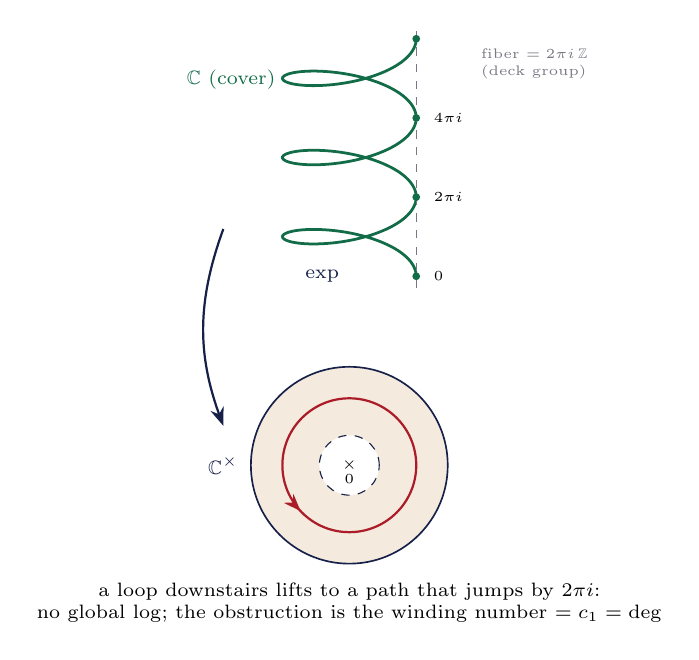
\begin{tikzpicture}
  % base C^* at the bottom
  \begin{scope}[shift={(0,-2.4)}]
    \fill[accent!14, even odd rule] (0,0) circle (1.25) (0,0) circle (0.38);
    \draw[inkblue, line width=0.6pt] (0,0) circle (1.25);
    \draw[inkblue, dashed, line width=0.4pt] (0,0) circle (0.38);
    \node[font=\tiny] at (0,0) {$\times$}; \node[font=\tiny, below=0pt] at (0,0){$0$};
    \draw[polered, loopdir, line width=0.8pt] (0,0) circle (0.85);
    \node[inkblue, font=\scriptsize] at (-1.6,0) {$\CC^\times$};
  \end{scope}
  % helix (the cover C via exp/log)
  \draw[zerogreen, line width=1pt, smooth, samples=140, domain=0:18.85]
        plot ({0.85*cos(\x r)}, {0.30*sin(\x r)+0.16*\x});
  \node[zerogreen, font=\scriptsize] at (-1.5,2.5) {$\CC$ (cover)};
  % fiber 2 pi i Z over z=1
  \draw[faint, dashed] (0.85,-0.15) -- (0.85,3.15);
  \foreach \k in {0,1,2,3}{ \fill[zerogreen] (0.85, {0.16*6.2832*\k}) circle (1.4pt); }
  \node[font=\tiny, right] at (0.95,0) {$0$};
  \node[font=\tiny, right] at (0.95,1.005) {$2\pi i$};
  \node[font=\tiny, right] at (0.95,2.01) {$4\pi i$};
  \node[font=\tiny, faint, right, align=left] at (1.55,2.7) {fiber $=2\pi i\,\ZZ$\\ (deck group)};
  % exp projection
  \draw[->, inkblue, line width=0.8pt] (-1.6,0.6) to[out=-110,in=110] (-1.6,-1.9)
        node[midway, left, font=\scriptsize] {$\exp$};
  \node[font=\scriptsize, align=center] at (0,-4.15)
    {a loop downstairs lifts to a path that jumps by $2\pi i$:\\
     no global $\log$; the obstruction is the winding number $=c_1=\deg$};
\end{tikzpicture}
\figcap{fig:expcover}{The exponential sequence $0\to\ZZ\to\OO\xrightarrow{\exp}
\OO^\times\to0$ made visible. The helix is the cover $\CC$; $\exp$ winds it down
onto $\CC^\times$ with fiber $2\pi i\,\ZZ$ (the constant sheaf $\ZZ$). A loop in
$\CC^\times$ lifts to a path that fails to close by a multiple of $2\pi i$, so the
obstruction to a global logarithm is exactly the winding number --- read by the
connecting map as $c_1=\deg$. (Supports \S10.)}
\end{center}

%=====================================================================
\section{Worked Micro-Examples}
%=====================================================================

\subsection*{Example A: \(S^1\) --- a disconnected overlap creates \(H^1\)}
Cover $S^1$ by two arcs $U,V$, each contractible, with $U\cap V$ \emph{two}
disjoint arcs $\simeq\{p\}\sqcup\{q\}$. Then $H^0(U)\oplus H^0(V)=\RR^2$ and
$H^0(U\cap V)=\RR^2$ (one $\RR$ per component). Mayer--Vietoris:
\[
  0\to H^0(S^1)\to \RR^2\xrightarrow{\,s\,}\RR^2\to H^1(S^1)\to
  \underbrace{H^1(U)\oplus H^1(V)}_{=0}.
\]
With constants $(a,b)$ on $(U,V)$, the difference on each overlap component is the
same value $a-b$, so
\[
  s(a,b)=(a-b,\ a-b),\qquad \kerop s=\{a=b\}\cong\RR,\qquad \im s=\{(t,t)\}\cong\RR .
\]
Hence $H^0(S^1)=\kerop s=\RR$ (connected), and
\[
  H^1(S^1)\cong\coker s=\RR^2/\{(t,t)\}\cong\RR .
\]
\diagnose{The $H^1$ of the circle is exactly the ``extra'' $\RR$ in
$H^0(U\cap V)=\RR^2$ caused by the overlap being \emph{disconnected}. The second
overlap component is where a global $1$-cocycle hides.}

\noindent Figure~\ref{fig:s1mv} makes the disconnected overlap visible.

\begin{center}
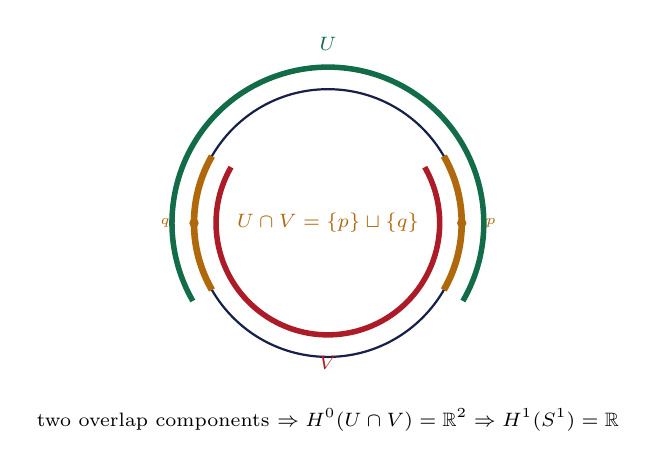
\begin{tikzpicture}
  \draw[inkblue, line width=0.8pt] (0,0) circle (1.7);
  \draw[zerogreen, line width=2pt] (-30:1.98) arc[start angle=-30, end angle=210, radius=1.98];
  \draw[polered,  line width=2pt] (150:1.42) arc[start angle=150, end angle=390, radius=1.42];
  \draw[accent, line width=2.4pt] (150:1.7) arc[start angle=150, end angle=210, radius=1.7];
  \draw[accent, line width=2.4pt] (-30:1.7) arc[start angle=-30, end angle=30, radius=1.7];
  \node[zerogreen, font=\scriptsize] at (90:2.28) {$U$};
  \node[polered,  font=\scriptsize] at (270:1.78) {$V$};
  \fill[accent] (0:1.7) circle (1.7pt);   \node[accent, font=\tiny, right] at (0:1.88) {$p$};
  \fill[accent] (180:1.7) circle (1.7pt); \node[accent, font=\tiny, left]  at (180:1.88) {$q$};
  \node[accent, font=\scriptsize] at (0,0) {$U\cap V=\{p\}\sqcup\{q\}$};
  \node[font=\scriptsize, align=center] at (0,-2.5)
    {two overlap components $\Rightarrow H^0(U\cap V)=\RR^2 \Rightarrow H^1(S^1)=\RR$};
\end{tikzpicture}
\figcap{fig:s1mv}{Mayer--Vietoris for $S^1$ with two arcs $U$ (outer, green) and
$V$ (inner, red). Their intersection has \emph{two} components $p,q$ (amber); the
``extra'' copy of $\RR$ in $H^0(U\cap V)=\RR^2$ is exactly what the connecting
map turns into $H^1(S^1)=\RR$. (Supports Example~A.)}
\end{center}

\subsection*{Example B: \(S^2\) --- the overlap circle detects the fundamental class}
Cover $S^2$ by two disks $U,V$ with $U\cap V\simeq S^1$ (an equatorial band).
This is the same shape as the $\PP^1$ cover. The relevant segment is
\[
  \underbrace{H^1(U)\oplus H^1(V)}_{0}\to H^1(S^1)=\RR\xrightarrow{\ \delta\ }
  H^2(S^2)\to \underbrace{H^2(U)\oplus H^2(V)}_{0},
\]
so $\delta\colon H^1(S^1)\xrightarrow{\cong}H^2(S^2)$, giving $H^2(S^2)=\RR$ and
\[
  \boxed{\ H^2(S^2)\cong H^1(S^1)\ }.
\]
\diagnose{The generator of $H^2(S^2)$ is the connecting image of the generator of
$H^1$ of the equatorial circle: the sphere's area class is the obstruction to
extending the circle's winding form over both caps (Section~9 makes the form
$d\rho_\infty\wedge\tfrac{d\theta}{2\pi}$ explicit).}

\noindent Figure~\ref{fig:capstone} summarizes this single step.

\begin{center}
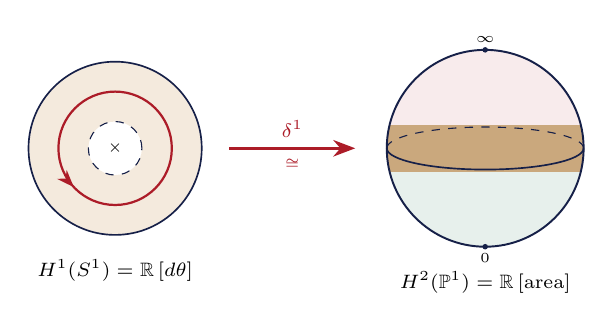
\begin{tikzpicture}
  % left: overlap circle with winding class
  \begin{scope}
    \fill[accent!14, even odd rule] (0,0) circle (1.1) (0,0) circle (0.34);
    \draw[inkblue, line width=0.6pt] (0,0) circle (1.1);
    \draw[inkblue, dashed, line width=0.4pt] (0,0) circle (0.34);
    \node[font=\tiny] at (0,0){$\times$};
    \draw[polered, loopdir, line width=0.8pt] (0,0) circle (0.72);
    \node[font=\scriptsize, align=center] at (0,-1.55) {$H^1(S^1)=\RR\,[d\theta]$};
  \end{scope}
  \draw[->, polered, line width=1.1pt] (1.45,0) -- (3.05,0)
        node[midway, above, font=\scriptsize, text=polered] {$\delta^1$}
        node[midway, below, font=\tiny] {$\cong$};
  % right: sphere with the area (H^2) class on the band
  \begin{scope}[shift={(4.7,0)}]
    \begin{scope}\clip (0,0) circle (1.25);
      \fill[zerogreen, fill opacity=0.10] (-1.25,-1.25) rectangle (1.25,0.3);
      \fill[polered,  fill opacity=0.09] (-1.25,-0.3) rectangle (1.25,1.25);
      \fill[accent,   fill opacity=0.45] (-1.25,-0.3) rectangle (1.25,0.3);
    \end{scope}
    \draw[inkblue, line width=0.7pt] (0,0) circle (1.25);
    \draw[inkblue, dashed, line width=0.4pt] (1.25,0) arc[start angle=0,end angle=180,x radius=1.25,y radius=0.27];
    \draw[inkblue, line width=0.6pt] (1.25,0) arc[start angle=0,end angle=-180,x radius=1.25,y radius=0.27];
    \fill[inkblue] (0,-1.25) circle (1pt); \node[font=\tiny,below=-1pt] at (0,-1.25){$0$};
    \fill[inkblue] (0, 1.25) circle (1pt); \node[font=\tiny,above=-1pt] at (0, 1.25){$\infty$};
    \node[font=\scriptsize, align=center] at (0,-1.7) {$H^2(\PP^1)=\RR\,[\mathrm{area}]$};
  \end{scope}
\end{tikzpicture}
\figcap{fig:capstone}{The whole document in one picture: the connecting
isomorphism $\delta^1$ carries the winding class on the overlap circle (left) to
the area class supported in the equatorial band of the sphere (right). The
obstruction to extending the circle's $1$-form over both caps \emph{is} the
fundamental class of $\PP^1=S^2$. (Supports Example~B; summarizes \S7--\S9.)}
\end{center}

\subsection*{Example C: \(\PP^1\) holomorphically --- \(dz/z\) and winding}
Use $U_0=\PP^1\setminus\{\infty\}$, $U_\infty=\PP^1\setminus\{0\}$,
$U_0\cap U_\infty=\CC^\times$. The overlap carries the meromorphic form $dz/z$,
whose period
\[
  \frac{1}{2\pi i}\oint_{|z|=1}\frac{dz}{z}=1
\]
records \emph{winding around $0$}. Two computations live on this overlap:
\begin{itemize}
  \item \emph{Constant sheaf / topology:} $[\,\tfrac{1}{2\pi i}\tfrac{dz}{z}\,]$
        generates $H^1_\dR(\CC^\times)$ and, via $\delta$, generates $H^2(\PP^1)$
        (Sections~8--9).
  \item \emph{Coherent sheaf $\OO$:} the \v Cech computation
        $\Hcech^1(\{U_0,U_\infty\},\OO)$ uses Laurent series. Every Laurent series
        $\sum_{n\in\ZZ}c_nz^n$ on $\CC^\times$ splits as
        \[
          \sum_{n\le0}c_nz^n\ \in\OO(U_\infty)\quad\text{minus}\quad
          \Bigl(-\sum_{n\ge1}c_nz^n\Bigr)\in\OO(U_0),
        \]
        so $\delta$ is surjective and $H^1(\PP^1,\OO)=\coker\delta=0$. Likewise
        $\kerop\delta=\{$global holomorphic$\}=\CC$ (Liouville), so
        $H^0(\PP^1,\OO)=\CC$.
\end{itemize}
\diagnose{The \emph{same} overlap $\CC^\times$ feeds two different sheaves: against
$\RR$ (topology) it produces the nonzero class detecting $H^2(\PP^1)$; against
$\OO$ (analysis) the Laurent splitting kills $H^1$. The discriminating data is
the coefficient sheaf, not the space.}

\subsection*{Example D: Line bundles --- cocycle, coboundary, and $\Hcech^1(\OO^\times)$}
A line bundle on $\PP^1$ is given by a single transition function
$g_{0\infty}\in\OO^\times(\CC^\times)$ (two charts, so the cocycle condition
$g_{\alpha\beta}g_{\beta\gamma}g_{\gamma\alpha}=1$ reduces to
$g_{\infty0}=g_{0\infty}^{-1}$; triple overlaps are empty). Now
\[
  \OO^\times(\CC^\times)=\{\,z^{n}e^{h(z)}:n\in\ZZ,\ h\in\OO(\CC^\times)\,\},
\]
and the coboundaries are $f_\infty/f_0$ with $f_0\in\OO^\times(U_0)=\{e^{h_0}\}$,
$f_\infty\in\OO^\times(U_\infty)=\{e^{h_\infty}\}$ (a nowhere-zero holomorphic
function on a contractible chart is an exponential). Splitting the Laurent series
$h=h_0+h_\infty$ as in Example~C, $e^{h}$ is a coboundary, so
\[
  g_{0\infty}=z^{n}e^{h}\ \sim\ z^{n},
\]
and the class is the integer
\[
  n=\frac{1}{2\pi i}\oint_{|z|=1}\frac{dg_{0\infty}}{g_{0\infty}}
   =\frac{1}{2\pi i}\oint_{|z|=1}d\log g_{0\infty}.
\]
Hence $\Hcech^1(\PP^1,\OO^\times)\cong\ZZ$ (matching Section~10's exponential
LES). With the convention $g_{0\infty}=z^{-d}$ of the divisor ledgers,
$n=-d$ and
\[
  \deg\OO(d)=-n=-\frac{1}{2\pi i}\oint_{|z|=1}d\log g_{0\infty}=d .
\]
\diagnose{The cocycle condition is the closedness ($\delta=1$) of a degree-$1$
multiplicative cochain; the coboundary freedom is exactly the change-of-trivialization
$h_\beta/h_\alpha$. The only surviving invariant is the winding number of the
transition function --- the degree.}

\noindent Figure~\ref{fig:linebundle} shows the cocycle and the $\PP^1$ gluing.

\begin{center}
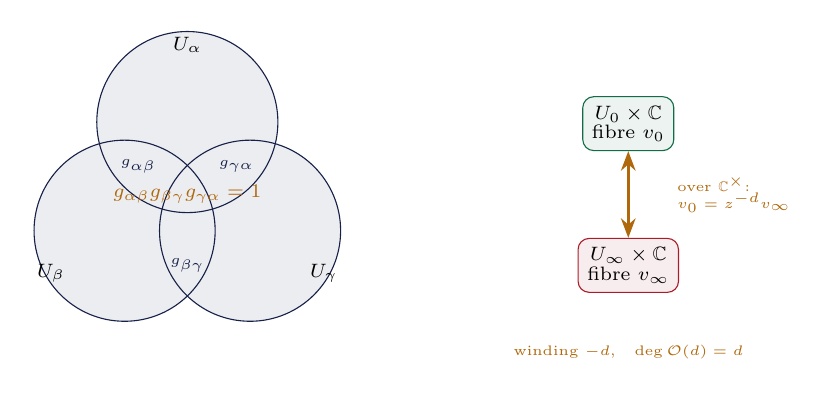
\begin{tikzpicture}
  % (a) cocycle on a triple overlap
  \fill[inkblue!8] (90:0.92) circle (1.15);
  \fill[inkblue!8] (210:0.92) circle (1.15);
  \fill[inkblue!8] (330:0.92) circle (1.15);
  \draw[inkblue] (90:0.92) circle (1.15);
  \draw[inkblue] (210:0.92) circle (1.15);
  \draw[inkblue] (330:0.92) circle (1.15);
  \node[font=\scriptsize] at (90:1.9) {$U_\alpha$};
  \node[font=\scriptsize] at (210:2.0) {$U_\beta$};
  \node[font=\scriptsize] at (330:2.0) {$U_\gamma$};
  \node[accent, font=\scriptsize, align=center] at (0,0) {$g_{\alpha\beta}g_{\beta\gamma}g_{\gamma\alpha}=1$};
  \node[font=\tiny, inkblue] at (150:0.72) {$g_{\alpha\beta}$};
  \node[font=\tiny, inkblue] at (270:0.9)  {$g_{\beta\gamma}$};
  \node[font=\tiny, inkblue] at (30:0.72)  {$g_{\gamma\alpha}$};
  % (b) the two-chart gluing on P^1
  \begin{scope}[shift={(5.6,0)}]
    \node[draw=zerogreen, rounded corners, fill=zerogreen!8, font=\scriptsize, align=center] (b0) at (0,0.9) {$U_0\times\CC$\\[-1pt]\scriptsize fibre $v_0$};
    \node[draw=polered, rounded corners, fill=polered!8, font=\scriptsize, align=center] (bi) at (0,-0.9) {$U_\infty\times\CC$\\[-1pt]\scriptsize fibre $v_\infty$};
    \draw[<->, accent, line width=0.9pt] (b0)--(bi);
    \node[font=\tiny, accent, right, align=left] at (0.5,0) {over $\CC^\times$:\\ $v_0=z^{-d}v_\infty$};
    \node[font=\tiny, accent, align=center] at (0,-2.0) {winding $-d$,\quad $\deg\OO(d)=d$};
  \end{scope}
\end{tikzpicture}
\figcap{fig:linebundle}{Line bundles as a degree-$1$ \v Cech class. \emph{Left}:
on a triple overlap the transition functions obey the cocycle condition
$g_{\alpha\beta}g_{\beta\gamma}g_{\gamma\alpha}=1$. \emph{Right}: on $\PP^1$ the
two trivial pieces are glued over $\CC^\times$ by $g_{0\infty}=z^{-d}$, whose
winding number $-d$ is the only invariant, giving $\deg\OO(d)=d$. (Supports
\S10, Example~D.)}
\end{center}

%=====================================================================
\section{Summary Table}
%=====================================================================
\begin{center}\footnotesize
\renewcommand{\arraystretch}{1.32}
\begin{tabular}{@{}p{2.05cm} p{2.55cm} p{2.75cm} p{3.0cm} p{3.4cm}@{}}
\toprule
\textbf{Tool} & \textbf{Input data} & \textbf{Algebraic form} &
\textbf{What it measures} & \textbf{Concrete meaning here}\\
\midrule
chain complex & forms / cochains \& a differential $d$ & $C^\bullet,\ d^2=0$ &
the apparatus in which ``closed'' and ``exact'' make sense &
$\Omega^\bullet(\PP^1)$; \v Cech $\CCech^\bullet(\{U_0,U_\infty\},\FF)$\\
cohomology & a chain complex & $H^n=\kerop d/\im d$ &
closed modulo exact (genuine obstructions) &
$H^\bullet_\dR(\PP^1)=(\RR,0,\RR)$; $H^\bullet(\PP^1,\OO)=(\CC,0)$\\
short exact sequence & sub/quotient of complexes & $0\!\to\!A\!\to\!B\!\to\!C\!\to\!0$ &
comparison of three worlds (global, local sum, overlap) &
$0\!\to\!\Omega^\bullet(X)\!\to\!\Omega^\bullet(U_0)\!\oplus\!\Omega^\bullet(U_\infty)\!\to\!\Omega^\bullet(\CC^\times)\!\to\!0$\\
connecting hom & a SES of complexes & $\delta\colon H^n(C)\!\to\!H^{n+1}(A)$ &
obstruction to lifting a closed class from $C$ to $B$ &
$\delta[d\theta]=$ generator of $H^2(\PP^1)$\\
long exact sequence & a SES of complexes & $\cdots\!\to\!H^n\!\to\!H^n\!\to\!H^n\!\xrightarrow{\delta}\!H^{n+1}\!\to\!\cdots$ &
how the three cohomologies constrain each other &
computes $H^\bullet(\PP^1)$; computes $\Pic$\\
Mayer--Vietoris & a cover $X=U\cup V$ & the LES of the cover SES &
global cohomology from local pieces $+$ overlap &
two disks $\cup$ annulus rebuild $S^2=\PP^1$\\
\v Cech cocycle & cover \& sheaf $\FF$ & $\{g_{\alpha\beta}\}$, $\delta g=0$ &
locally trivial data compatible on overlaps &
transition $g_{0\infty}\in\OO^\times(\CC^\times)$ of a line bundle\\
coboundary & a $0$-cochain & $g_{\alpha\beta}=h_\beta/h_\alpha$ &
data that is a re-trivialization, hence trivial &
change of chart $e^{h_\infty}/e^{h_0}$; winding $0$\\
gluing obstruction & cocycle mod coboundary & $H^1(X,\FF)$ &
failure of local data to be global &
$\Hcech^1(\OO^\times)=\Pic(\PP^1)=\ZZ$ (the degree)\\
\bottomrule
\end{tabular}
\end{center}

%=====================================================================
\section{Final Conceptual Diagram}
%=====================================================================
The whole pipeline, with the Mayer--Vietoris branch feeding the short exact
sequence that drives everything.

\begin{center}
\resizebox{\textwidth}{!}{%
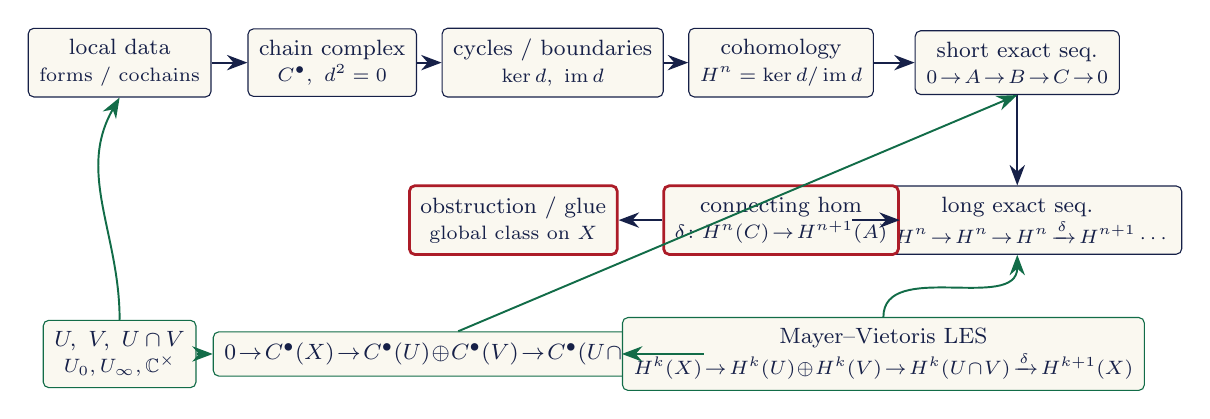
\begin{tikzpicture}[
  >={Stealth[length=2.6mm]},
  box/.style={draw=inkblue, rounded corners=2pt, fill=paper, align=center,
              inner sep=4pt, font=\footnotesize, text=inkblue},
  mv/.style={draw=zerogreen, rounded corners=2pt, fill=paper, align=center,
              inner sep=4pt, font=\footnotesize, text=inkblue},
  hi/.style={draw=polered, line width=1pt, rounded corners=2pt, fill=paper,
              align=center, inner sep=4pt, font=\footnotesize, text=inkblue},
  ar/.style={->, inkblue, line width=0.7pt},
  arg/.style={->, zerogreen, line width=0.7pt}
]
  % main pipeline (top row)
  \node[box] (loc) at (0,0)      {local data\\ \scriptsize forms / cochains};
  \node[box] (cx)  at (2.7,0)    {chain complex\\ \scriptsize $C^\bullet,\ d^2=0$};
  \node[box] (zb)  at (5.5,0)    {cycles / boundaries\\ \scriptsize $\kerop d,\ \im d$};
  \node[box] (coh) at (8.4,0)    {cohomology\\ \scriptsize $H^n=\kerop d/\im d$};
  \node[box] (ses) at (11.4,0)   {short exact seq.\\ \scriptsize $0\!\to\!A\!\to\!B\!\to\!C\!\to\!0$};
  \node[box] (les) at (11.4,-2.0){long exact seq.\\ \scriptsize $\cdots H^n\!\to\!H^n\!\to\!H^n\!\xrightarrow{\delta}\!H^{n+1}\cdots$};
  \node[hi]  (con) at (8.4,-2.0) {connecting hom\\ \scriptsize $\delta\colon H^n(C)\!\to\!H^{n+1}(A)$};
  \node[hi]  (obs) at (5.0,-2.0) {obstruction / glue\\ \scriptsize global class on $X$};

  \draw[ar] (loc)--(cx);
  \draw[ar] (cx)--(zb);
  \draw[ar] (zb)--(coh);
  \draw[ar] (coh)--(ses);
  \draw[ar] (ses)--(les);
  \draw[ar] (les)--(con);
  \draw[ar] (con)--(obs);

  % Mayer-Vietoris branch (bottom row) feeding the SES
  \node[mv] (uvw) at (0,-3.7)  {$U,\ V,\ U\cap V$\\ \scriptsize $U_0,U_\infty,\CC^\times$};
  \node[mv] (mvses) at (4.3,-3.7) {$0\!\to\!C^\bullet(X)\!\to\!C^\bullet(U)\!\oplus\!C^\bullet(V)\!\to\!C^\bullet(U\!\cap\!V)\!\to\!0$};
  \node[mv] (mvles) at (9.7,-3.7) {Mayer--Vietoris LES\\ \scriptsize $H^k(X)\!\to\!H^k(U)\!\oplus\!H^k(V)\!\to\!H^k(U\!\cap\!V)\!\xrightarrow{\delta}\!H^{k+1}(X)$};

  \draw[arg] (uvw)--(mvses);
  \draw[arg] (mvses)--(mvles);
  \draw[arg] (uvw.north) to[out=90,in=-120] (loc.south);
  \draw[arg] (mvses.north) -- (ses.south);
  \draw[arg] (mvles.north) to[out=90,in=-90] (les.south);
\end{tikzpicture}}
\end{center}

\noindent
\textbf{Reading.} The top row is the abstract machine: local data assemble into a
chain complex; the differential carves out cycles and boundaries; their quotient
is cohomology; a comparison of complexes is a short exact sequence; its shadow on
cohomology is the long exact sequence, whose connecting map is the obstruction
that becomes a global class. The green Mayer--Vietoris branch is the geometric
instantiation: cutting $\PP^1$ into $U_0,U_\infty$ with overlap $\CC^\times$ is
\emph{exactly} the short exact sequence that drives the machine, and its
connecting map manufactures $H^2(\PP^1)$ and (via $\OO^\times$) the degree of a
line bundle.

\slogan{Homological algebra is not formal machinery. It is a controlled way to
watch local data become global structure --- and to measure, as a single
cohomology class, precisely where the gluing fails.}

\end{document}
